\section{Evaluation}

A large challenge in creating quality measures is the
problem of evaluating the performance of the measure.
``Quality'' is an imprecise notion by itself, because it
necessarily must be evaluated with respect to some attribute.
For example, within the Wikipedia we might evaluate the quality
of a contribution along any of these dimensions:
\begin{itemize}
\item grammar
\item diction
\item neutral point of view
\item factual correctness
\end{itemize}
Our text and edit longevity measures try to go one step
further into the fuzzy world of human evaluations by using
later edits as a basis for inferring sentiment about earlier edits.
Is this a valid inference to make?
How can such a question be answered?

The surest way to measure sentiment would be to interview
users as they are making edits to the Wikipedia and documenting
their thought processes as they read an article and make the
decision to edit an article --- but this would require an enormous
effort to collect enough data for performance evaluation.
We propose that we can grossly measure the sentiment of the
community by recognizing that there is a generally agreed upon
standard of articles being of ``encyclopedic quality''
which allows people to recognize vandalism when they see it.
Accepting that premise allows us to use the PAN-WVC-10
corpus~\cite{Potthast2010a} as a manually annotated data set for
such an evaluation.

A complication in our evaluation is our restricted setting of
\textit{filtered} revisions, where sequential revisions by the
same author are filtered out to leave only the last revision
in the sequence.
This would limit us in evaluating the performance of our
quality measures, so we modified the system in the following way:
we do not filter revisions annotated in the PAN-WVC-10 corpus,
or the immediately preceding revision (even when they have the
same author), but we do filter revisions \textit{after} the annotated
revision in the usual way.
Even with this loosening of the revision filtering, several
revisions are still not evaluated for quality; the two
primary reasons for no evaluation are a lack of subsequent
edits to base the evaluation on, or the revision was not
substantially different from the previous revision
(that is, $\dist{}{k-1,k} = 0$, which can happen when only
whitespace changes).

The PAN-WVC-10 corpus contains 32,439 edits, where each revision was
manually reviewed by at least three annotators to assign a label
of either ``regular'' or ``vandalism.''
We used the dump of the English Wikipedia from January 30, 2010
to extract the text of each annotated revision, along with the revision
before and the ten filtered revisions following so that we could compute
our text longevity and edit longevity measures for each annotated edit.
Out of the total 32,439 revisions, we were able to compute
edit longevity scores for 27,730 revisions, and text longevity
scores for 28,453 revisions.

We used the straight-forward transformation to convert
each quality score from its normal range into the range
$[0,1]$, to be interpreted as a probability that the named
revision was the result of vandalism.
As in the PAN 2010 competition~\cite{Potthast2010b}, we use the
\texttt{perf}\footnote{\url{http://kodiak.cs.cornell.edu/kddcup/software.html}}
package to evaluate the performance of our quality measures
by computing the area under the receiver operating characteristic
curve \footnote{\url{http://en.wikipedia.org/wiki/Receiver_operating_characteristic}},
and also the mean precision value.

\mynote{Bad triangles; how many?}


\begin{table}[htbp]
\begin{center}
\begin{tabular}{|r|c|c|c|c|c|}
\cline{3-6}
\multicolumn{2}{c|}{} & \multicolumn{2}{|c|}{Text Longevity} & \multicolumn{2}{|c|}{Edit Longevity} \\
\hline
Diff & Edit Distance & ROC AUC & Mean Prec. & ROC AUC & Mean Prec. \\
\hline
\hline
basic & initial distance & xx & xx & xx & xx \\
basic & updated distance & xx & xx & xx & xx \\
live & I+D+M & 85.949\% & 29.235\% & 91.758\% & 44.052\% \\
live & graph & 85.949\% & 29.235\% & 91.761\% & 46.539\% \\
\hline
\end{tabular}
\end{center}
\caption{Comparison of the performance of text and edit longevity
  using three different definitions of edit distance.
  The edit quality computed was used as a predictor for the probability
  that annotated revisions from the PAN-WVC-10 corpus were vandalism.
  Each measure is evaluated by computing the area under the
  receiver operating characteristic (ROC) curve.
} 
\label{tbl:editquality}
\end{table}


Why does text longevity not do so well as edit longevity?
As part of our investigation, we started looking at specific
instances of text longevity values.
In Figures~\ref{fig:ts-GeorgeWBush} and~\ref{fig:ts-SantaCruzBeachBoardwalk},
we see the text survival for two different contributions;
both do seem to have the general ``exponential'' shape
that we previously described.
Also computed in each figure is the text longevity metric based on
the 20~revisions shown in each graph, but notice that the text
longevity computed for
Figure~\ref{fig:ts-GeorgeWBush} doesn't exhibit curve we expect.

\begin{figure}[tbph]
\centering
\framebox{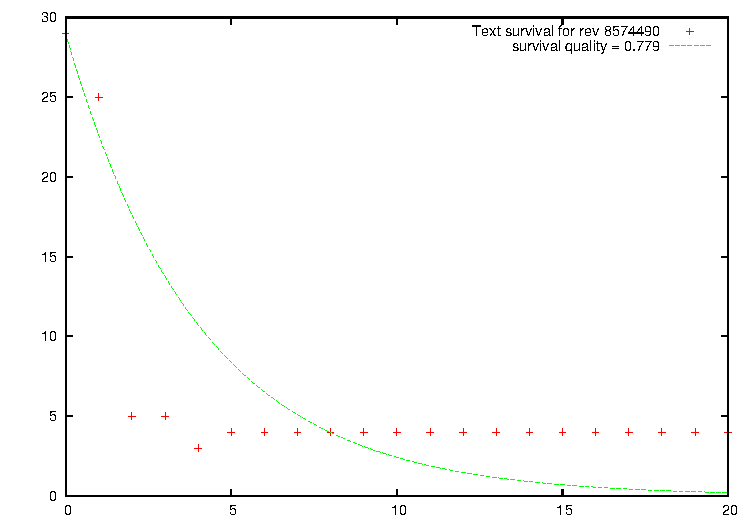
\includegraphics[width=0.8\textwidth]{part-F70-editquality/graph-TS-GeorgeWBush-8574490}}
\caption{The text survival graph for the text contributed early
        in the history of article \textit{George W.~Bush}.
	The graph also shows the text survival quality
	computed based on 20~revisions.
	}
\label{fig:ts-GeorgeWBush}
\end{figure}

\begin{figure}[tbph]
\centering
\framebox{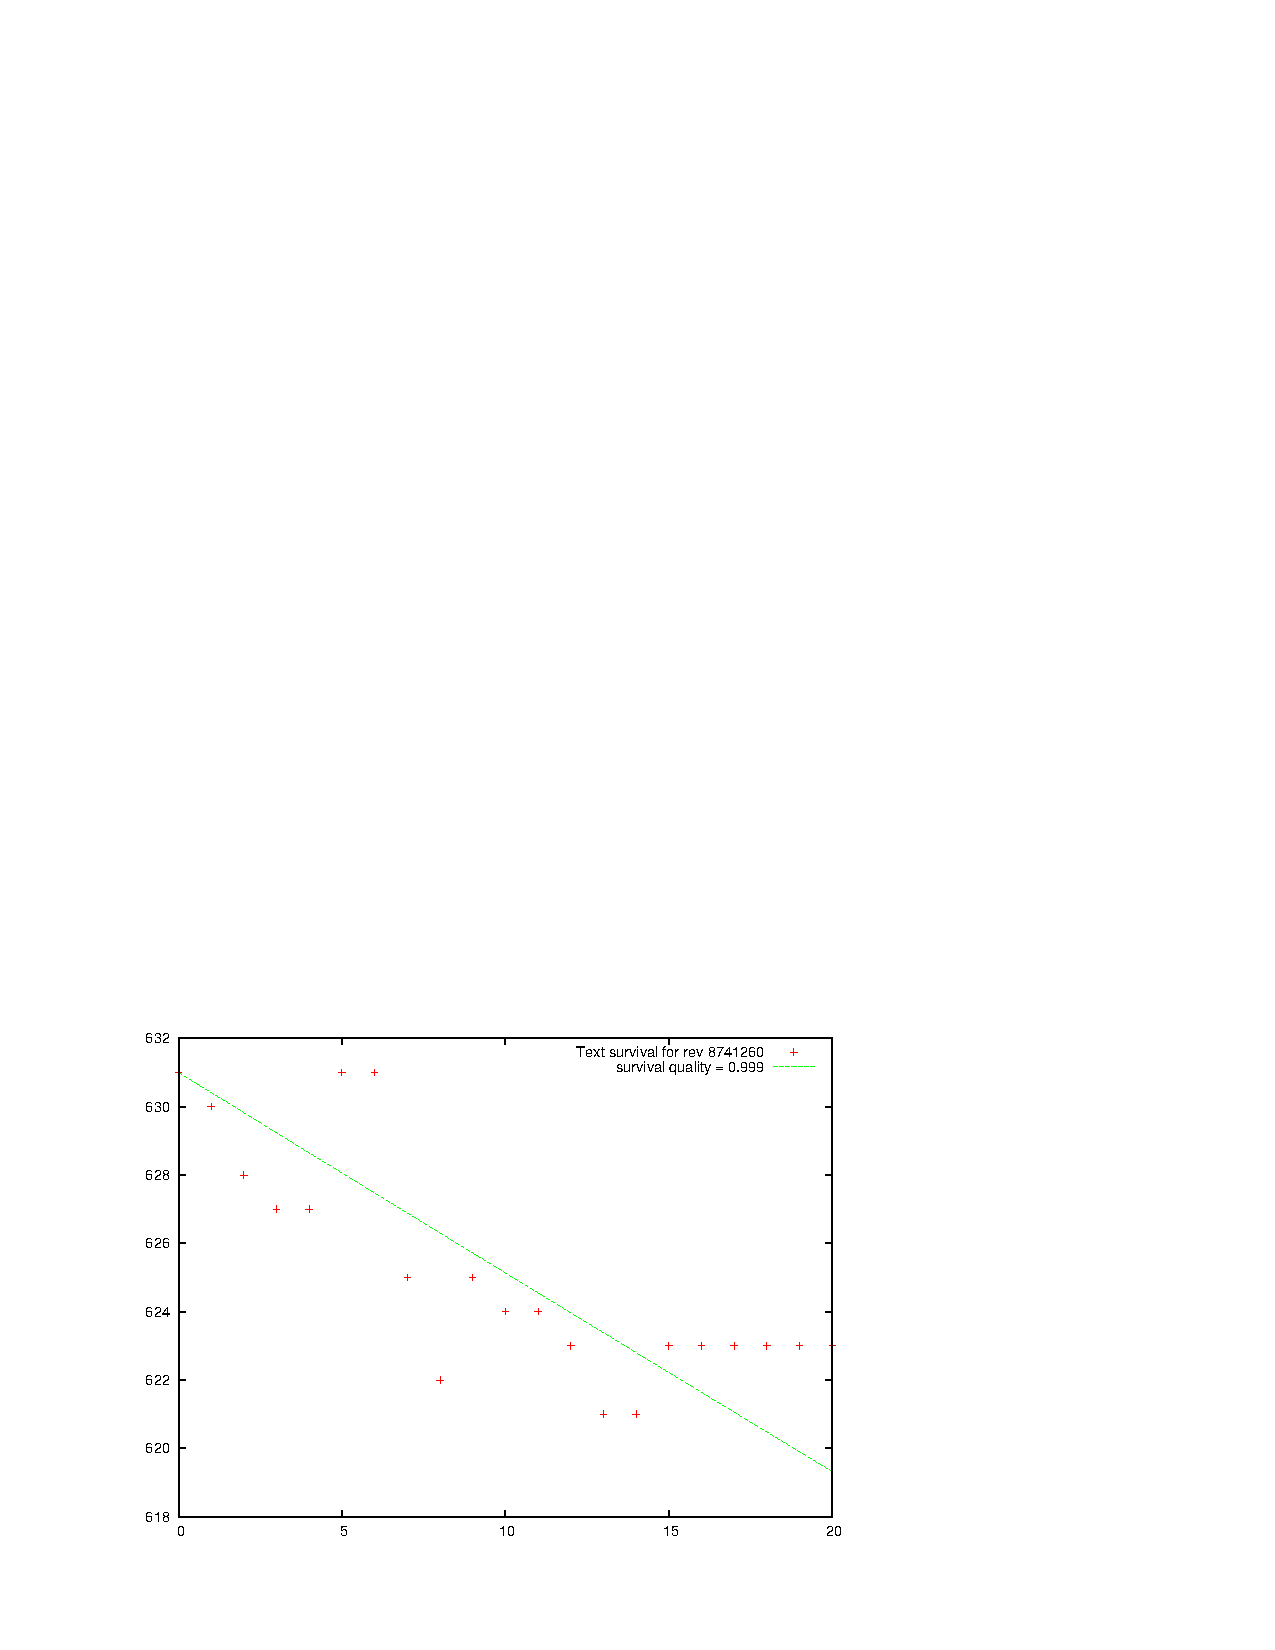
\includegraphics[width=0.8\textwidth]{part-F70-editquality/graph-TS-SantaCruzBeachBoardwalk}}
\caption{The text survival graph for the text initially contributed
	as part of the article \textit{Santa Cruz Beach Boardwalk}.
	The majority of the editing to the contributed text happens
	in the next few revisions, before the text stabilizes.
	The graph also shows the text survival quality
	computed based on 20~revisions.
	}
\label{fig:ts-SantaCruzBeachBoardwalk}
\end{figure}

The explanation for this discrepancy turns out to be a flaw in our
thinking about the original model.
While the text survival for contributions does seem to have an
exponential look to it, exponentials do not approach some fixed
non-zero value --- they approach zero.
In order to fit the curve we are describing, the last value
(in the case of the data shown in Figure~\ref{fig:ts-GeorgeWBush},
the amount of text that survives after the $20^{th}$ revision)
should be taken as the ``zero reference point'' which is subtracted
from all the values.
Applying our exponential curve fitting technique to these new values
will give a much better approximation to the data.
The problem with this better fit is that it changes the meaning of
a score of zero; instead of meaning that the text was immediately deleted,
a score of zero would mean that the text immediately reached its
final survival level.
In other words, we would be measuring how quickly the text stabilizes,
rather than how much agreement there was that the text belonged in
the article.

\subsection{The Triangle Inequality}

We previously noted that our formulation of edit longevity does
not precisely stay within the desired range of $[-1,+1]$,
because our use of a greedy differencing algorithm does not
guarantee the shortest edit script.
In order to quantify how often such an error might crop up,
we counted how many triangles were evaluated for our PAN-WVC-10
revisions, and how many of those fell outside of the range $[-1,+1]$.

\begin{table}[htbp]
\begin{center}
\begin{tabular}{|r|c|c|c|}
\hline
Diff & Edit Distance & Total Triangles & Bad Triangles \\
\hline
\hline
basic & initial distance & xx & xx \\
basic & updated distance & xx & xx \\
live & I+D+M & 850,060 & 46,740 \\
live & graph & 852,040 & 162,922 \\
\hline
\end{tabular}
\end{center}
\caption{Estimating how often the triangle inequality does
    not hold when evaluating edit longevity of the
    PAN-WVC-10 annotated revisions.
} 
\label{tbl:badtriangles}
\end{table}


